% LaTeX file for resume 
% This file uses the resume document class (res.cls)
\documentclass[margin,line]{res} 
\usepackage{hyperref}
\usepackage[export]{adjustbox}
\usepackage{wrapfig}
\usepackage{lipsum}

\setlength{\topskip}{0mm}
\setlength{\parindent}{1mm}
\oddsidemargin -.5in
\evensidemargin -.5in
\textwidth=6.0in
\itemsep=0in
\parsep=0in
\topmargin=-0.5in
\topskip=-0.5in
\textheight 9.5in

\newcommand{\MySlogan}[1]{ % Slogan}{optional)
		\large \usefont{OT1}{phv}{m}{n}\hfill \textit{#1}
		\par \normalsize \normalfont}

\newcommand{\MyName}[1]{ % Name
		\Huge \usefont{OT1}{phv}{b}{n} \hfill #1
		\par \normalsize \normalfont}
% the margin option causes section titles to appear to the left of body text 
%\textwidth=5.2in % increase textwidth to get smaller right margin
%\usepackage{helvetica} % uses helvetica postscript font (download helvetica.sty)
%\usepackage{newcent}   % uses new century schoolbook postscript font 

\begin{document} 


% \thispagestyle{empty} % this page has no header  
% \begin{tabular}{@{}p{3.5in}p{3in}}
% {\bf Contact Information:}
% \\39 West Lexington Street, \\803             
% Baltimore, MD, 21201
%  \\{Phone:}  (443) 653-7320 \\
%  {E-mail:}  zahranoorcs1514@gmail.com\\

% \end{tabular}
% \hfill
% 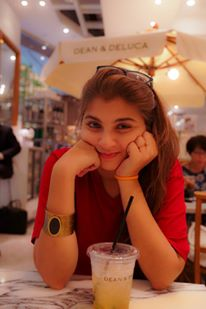
\includegraphics[width=3cm,valign=t]{mypic.jpg}%
% %\name{Zahra Noor\\[12pt]} % the \\[12pt] adds a blank line after name
% \name{\LARGE Zahra Noor}


\begin{wrapfigure}{l}{0.5\textwidth}
	\vspace*{-2em}
	\hspace*{-10em}
		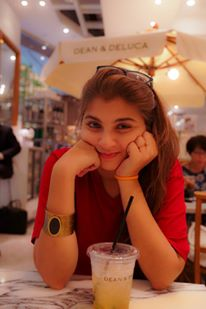
\includegraphics[width=0.15\textwidth]{mypic.jpg}
\end{wrapfigure}

\MyName{Zahra Noor}
% \MySlogan{Curriculum Vit\ae\ (\today)}
\MySlogan{Web Developer}
\MySlogan{\vspace{-0.6in}\begin{flushright}{}{39 West Lexington Street}\\803, Baltimore, MD, 21201 \\
(443) 653-7320\\
E-mail: zahranoorcs1514@gmail.com\\
\MySlogan{Portfolio: \href{https://zahranoorcs.github.io/MyPortfolio/index.html}{\bf Click here}}
\end{flushright}}


\begin{resume} 
 
% \section{\bf Contact Information}
% \vspace{.05in}
% \begin{tabular}{@{}p{3.5in}p{3in}}
% 39 West Lexington Street, \\803             
% Baltimore, MD, 21201
%  \\{Phone:}  (443) 653-7320 \\
%  {E-mail:}  zahranoorcs1514@gmail.com\\

% \end{tabular}

\section{Career \\Objective}

Seeking a job as a web application developer/front-end web developer which will utilize my skills for the growth of the organization while providing me an opportunity for mutual growth and advancement.

\section{Professional \\Experience}

\href{http://www.datanext.co.jp/en/}{\bf DataNext Corporation Ltd}, Naha, Okinawa. Japan. \hfill{June 2016 -- March 2017}\\
Web Developer
\begin{itemize} \itemsep -2pt  % reduce space between items
 \item Developing a web-based application as a real-time aid for product delivery staff to generate reports and for managers to monitor delivery schedule, delivery location, work efficiency etc using Laravel as framework.
 The app included additional features for delivery staff to make their delivery schedule, routing and sorting more easy.
 \item Utilized HTML, CSS, JavaScript, PHP, AngularJS and AJAX to create Web-based application. 
 \item Converting mockups into HTML and CSS.
 \item Increasing responsiveness of webpages using bootsrtrap.
 \item Analyzing software usability and performance, recommending changes to improve functionailty.
 \item Testing site functionality and identifying problems.
 \item Some experience in creating mock-ups and presentations.
 \item Collaborating with team in order to conduct function-based brainstorming. 

 \end{itemize}
{\bf Microsoft Innovation Center (MIC)}, Lahore \hfill 
Summer 2014\\
 Development Intern
\begin{itemize} \itemsep -2pt  % reduce space between items
 \item Developing Natural Language Processing applications for windows\\based systems using C\# 
 \end{itemize}
  \href{https://lums.edu.pk/}{\bf Lahore University of Management Science(LUMS)}, Lahore \hfill Summer 2013
\\Research Intern
\begin{itemize} \itemsep -2pt  % reduce space between items
 \item Support Vector Machine based Algorithms for outliers detection from\\real-time data 
 \end{itemize}


\section{Technical \\Skills}
{\bf Programming Languages and Softwares}: HTML(Intermediate), CSS(Intermediate),\\  JavaScript(Intermediate), PHP(Intermediate), Bootstrap(Intermediate), jQuery(Novice), \\AngularJS(Novice), Python(Novice)
\\{\bf Tools}: Microsoft Office, Laravel, Wordpress, Navicat for MySQL

\section{Education} 
\href{http://www.lcwu.edu.pk/}{\bf Lahore College for Women University(LCWU)}, Lahore \hfill 2010 -- 2014\\ B.S. Computer Science \hfill(GPA 3.48/4.0)
\begin{itemize} \itemsep -2pt  % reduce space between items
 \item Senior Year Project: Idea Market: An Android based ideation system
 \item  Major Courses: Artificial Intelligence, Human Computer Interaction,\\ Computer Graphics, Operating Systems 
 \end{itemize}

\section{Continuing \\Education}
{\bf Coursera:} HTML, CSS, and Javascript for Web Developers(Johns Hopkins University)\\
{\bf Udacity:} Full Stack Web Developer Nanodegree Program(Course in Progress)

\section{Availability}
Available from July 21st, 2017
\section{Refrences}
\begin{itemize} \itemsep -2pt  % reduce space between items
  \item {\bf Mr. Higa Satoshi,}\\
  Technical Leader, DataNext Corporation Ltd \\
  E-mail: s.higa@datanext.co.jp \\



  \item {\bf Mr. Tran Minh Nhut,}\\
  Senior Web Developer, DataNext Corporation Ltd \\
  E-mail: minhnhut37@gmail.com \\

\end{itemize}

\end{resume} 
\end{document} 



